\documentclass{article}
\usepackage{graphicx}
\graphicspath{ {images/} }
\usepackage[utf8]{inputenc}
\usepackage[spanish]{babel}
\usepackage[letterpaper,top=2cm,bottom=2cm,left=3cm,right=3cm,marginparwidth=1.75cm]{geometry}

\usepackage{fancyhdr}
\usepackage{hyperref}
\usepackage{listings}
\lstset{language=Python}

\pagenumbering{arabic}
\title{Manejo de datos en Phyton}
\author{Juan Andrés Silva Rodriguez }
\date{June 2021}


\begin{document}

\maketitle

\section{Predicción de casillas}

\subsection{Metodología}
Para la predicción de casillas que con anterioridad se había realizado en \textit{Excel} se usaron las librerías pertinentes: pandas, especializada en el manejo y análisis de estructuras de datos, y tal. Asimismo, se utilizó una función encontrada en línea para eliminar aquellas columnas del dataframe que sean diferentes a las definidas.\\

Se inició guardando las direcciones de todos los archivos .csv correspondientes a las listas nominales de los meses comprendidos entre sep/2019 y dic/2020, obtenidos en la página web del INE \cite{Data}, en una sola lista. Posteriormente, se inició un ciclo \textit{for} necesario para convertir todos los archivos guardados en all\_files a dataframes, así como para hacer las siguientes modificaciones (en orden cronológico):
\begin{enumerate}
    \item Eliminar las filas donde la columna de \textsc{entidad} sea diferente de 11 (el número asignado al estado de guanajuato).
    
    \item Cambiar el nombre de las columnas de LISTA a TOTAL\_LISTA, ya que en algunos archivos varía esta etiqueta y se necesitó cohesión en los nombres para evitar conflictos de compilación.
    
    \item Eliminar todas las columnas a excepción de TOTAL\_LISTA y SECCION, ya que son los unicos dos datos necesarios para nuestro análisis.
\end{enumerate}

\begin{lstlisting}
path = r'C:\Users\joana\Desktop\INE' # use your path
all_files = glob.glob(path + "/*.csv")
li = []
i=0
for filename in all_files:
    df = pd.read_csv(filename, thousands=r',', index_col=None, header=0)
    indexNames = df[ df['ENTIDAD'] != 11 ].index
    df.drop(indexNames , inplace=True)
    df = df.rename(columns = {'LISTA': 'TOTAL_LISTA'}, inplace = False)
    if (i==0):
        remove_others(df, {"SECCION", "TOTAL_LISTA"})
        df = df.sort_values(by=['SECCION'])
        df = df.iloc[:3142,:]
    else:
        remove_others(df, {"SECCION", "TOTAL_LISTA"})
        df = df.sort_values(by=['SECCION'])
        remove_others(df, {"TOTAL_LISTA"})
        df = df.iloc[:3142,:]
        
    li.append(df)
    i=1
\end{lstlisting}
    
\clearpage

El conjunto de dataframes obtenidos en el ciclo \textit{for} se concatenan en \textit{frame}.

\begin{lstlisting}    
frame = np.append(li[0], li[1], axis=1)
j =2
for i in range(14):
    frame = np.append(frame, li[j], axis=1)
    j = j+1        
\end{lstlisting}

Al finalizar lo anterior, se aplicó la función de regresión lineal utilizando un codigo encontrado en internet\cite{pag} con un vector X conteniendo los valores del 1 al 16 (secuencia de continuidad de los meses de la base de datos), y en un ciclo for se fue redefiniendo el valor de y por cada linea del dataframe "frame". Se predijo el numero de votos para el mes 18 siendo este Febrero del 2021 por cada seccion y este numero se dividio entre 750 para asi obtener el numero de casillas por seccion, finalmente se sumaron el numero de casillas con la funcion sum() y este dato se imprime.

\begin{lstlisting}
x = np.array([1,2,3,4,5,6,7,8,9,10,11,12,13,14,15,16])
regresion_lineal = LinearRegression()
predicciones = []
for i in range (len(frame)):

    y = frame[i, 1:].reshape(-1,1
    regresion_lineal.fit(x.reshape(-1,1), y) 
    nuevo_x = np.array([18]) 
    predicciones.append(math.ceil(float
    (regresion_lineal.predict(nuevo_x.reshape(-1,1)))))
    
del predicciones[0]
casillas = []

for prediccion in predicciones:
    casillas.append(math.ceil(prediccion/750))

print(sum(casillas))
\end{lstlisting}

\subsection{Resultados}
Como resultado se obtuvo la predicción del numero de casillas a instalar por sección para Febrero del 2021 siendo este de 7562. La gráfica de regresión lineal era demasiado complicada de imprimir dado que sería una por sección y estas son aproximadamente 3000 por lo que únicamente se imprimió como resultado final la sumatoria de casillas a instalar.

\subsection{Conclusión}
El análisis de esta base de datos fue un poco mas complicada de lo que esperaba en comparación a la realizada en \textit{Excel}, algunos de los datos de los archivos .csv contenían comas para separar los miles lo cual dificulto su lectura, aun así, considero que \textit{Python} es una herramienta mas completa y multifacética a diferencia de la simplicidad de su contra-parte \textit{Excel} en este proyecto.

\clearpage
\section{Indicadores de obesidad}

\subsection{Introducción}
La segunda base de datos se obtuvo de ICU Machine Learning Repository, titulada "Estimation of obesity levels based on eating habits and physical condition'' \cite{obs}, con la que se buscó realizar un método de determinación de la clasificación de los niveles de obesidad distinto al ya conocido con el índice de masa corporal.

Se optó por usar un aprendizaje supervisado, método aprendido en la clase de \textit{Machine Learning} de este semestre; el machine learning es el estudio de algoritmos computacionales que se optimizan automáticamente a través de la experiencia y el uso de información \cite{lib}. Por otro lado, el aprendizaje supervisado son algoritmos que aprenden a través de etiquetas de clase provistas por el usuario.

El aprendizaje supervisado puede aplicarse a diversos problemas como la clasificación. Para efectos de este trabajo se eligieron dos clasificadores:
\begin{itemize}
    \item K-nearest neighbores: Funciona buscando los "vecinos mas cercanos", siendo estos los puntos mas cercanos basándonos en algún tipo de distancia, en este caso se utilizó la distancia euclidiana, dados los vecinos mas cercanos se selecciona la etiqueta de clase mas repetida entre estos y es la elegida para el nuevo punto.
    \item Supported Vector Machine: Este clasificador aplica un modelo matemático de minimización para encontrar el hiper-plano que mejor logre separar las clases, en este caso se utilizo un parámetro kernel (rbf) el cual mapea los puntos en un nuevo espacio de mayor dimensionalidad en la que la separación sea mas evidente y una vez encontrado el plano se regresa a la dimensionalidad original.
\end{itemize}

\subsection{Metodología}
Las librerías utilizadas se muestran acá abajo. Las ultimas tres importaciones son propias de la librería \textit{sklearn}, ésta cuenta con algoritmos óptimos para la clasificación.

\begin{lstlisting}
import numpy as np
import pandas as pd
from typing import Set, Any 
from sklearn.preprocessing import StandardScaler
from sklearn.svm import SVC
from sklearn.neighbors import KNeighborsClassifier
import matplotlib.pyplot as plt
\end{lstlisting}

Se encontró una función para remover las columnas del dataframe a excepción de las definidas por el usuario. Además, se lee el archivo .csv y se guarda en el dataframe df.
\begin{lstlisting}
def remove_others(df: pd, columns: Set[Any]):
    cols_total: Set[Any] = set(df.columns)
    diff: Set[Any] = cols_total - columns
    df.drop(diff, axis=1, inplace=True)

df = pd.read_csv("ObesityDataSet_raw_and_data_sinthetic.csv")
\end{lstlisting}

Posteriormente, se usa la función definida arriba para remover todas las columnas del dataframe, a excepción de \textit{Weight}, \textit{Height}, \textit{NObeyesdad}, que son los necesarios para el análisis. En adición, se reemplazan todas las etiquetas de clase del dataset por valores numéricos, para hacer más fácil la clasificación. Finalmente, se guardaron los datos modificados en otro archivo .csv, ya que para mayor facilidad de uso del código utilizado para la graficación de los clasificadores era mas sencillo reescribir los datos.
\clearpage
\begin{lstlisting}
remove_others(df, {"Weight", "Height", "NObeyesdad"})

df=df.replace(to_replace="Insufficient_Weight",value="0")
df=df.replace(to_replace="Normal_Weight",value="1")
df=df.replace(to_replace="Overweight_Level_I",value="2")
df=df.replace(to_replace="Overweight_Level_II",value="2")
df=df.replace(to_replace="Obesity_Type_I",value="3")
df=df.replace(to_replace="Obesity_Type_II",value="4")
df=df.replace(to_replace="Obesity_Type_III",value="5")

df.to_csv("asd.csv",index=False)
\end{lstlisting}

Se declaran los clasificadores y sus parámetros correspondientes, los parámetros son los estandarizados para problemas de clasificación simple.

\begin{lstlisting}
names = ["Nearest Neighbors", "SVC (RBF)"]
classifiers = [KNeighborsClassifier(5), SVC(kernel="rbf", C=10, gamma =0.1),]
\end{lstlisting}

Se lee el dataset modificado y almacenado en el dataframe y se redefine como tupla (formato mas eficiente para el código de gráficas). Se declara una lista con varios arreglos con altura y peso que serán puntos de prueba para los algoritmos ya entrenados.
\begin{lstlisting}
data = []
with open('asd.csv', newline='') as csvfile:
    next(csvfile)
    df = pd.read_csv(csvfile, sep=',', names=["x1", "x2", "y"])
    data.append([df.values[:, 0:2], df.values[:, 2]])
    
data = tuple(data[0])

my_imc = [[1.7, 50],[1.77,92],[1.6,120],[1.62,60],[1.56,130],[1.6,95],
[1.75, 110],[1.59,84],[1.69,60],[1.72, 76],[1.69,82],[1.75,70],[1.67,50],
[1.55,92],[1.77,70]]
\end{lstlisting}

Se declara la figura en la que se guardaran las gráficas y la separación que habrá entre estas en ella. Posteriormente, se definieron los valores de X (peso y altura) que cumplen la función de par ordenados para la gráfica y y las etiquetas de clase. Y asignación de variables que serán utilizadas para crear las fronteras de decisión.
\begin{lstlisting}
figure = plt.figure(figsize=(12,5))
h = .02  
X, y = data
X = np.append(X, my_imc, axis = 0)
X = StandardScaler().fit_transform(X)
X12 = X[-len(my_imc): ]
X = (np.delete(X, slice(-(len(my_imc)+1), -1), 0))
X_train, y_train = X , y
x_min, x_max = X[:, 0].min() - .5, X[:, 0].max() + .5
y_min, y_max = X[:, 1].min() - .5, X[:, 1].max() + .5
xx, yy = np.meshgrid(np.arange(x_min, x_max, h), np.arange(y_min, y_max, h))
ax = plt.subplot(1, len(classifiers) + 1, 1)
ax.set_title("Input data")
scatter=ax.scatter(X_train[:, 0], X_train[:, 1], c=y_train, edgecolors='k')
ax.set_xlim(xx.min(), xx.max())
ax.set_ylim(yy.min(), yy.max())
ax.set_xticks(())
ax.set_yticks(())
legend1 = ax.legend(*scatter.legend_elements(), loc="upper left", title="Classes")
i = 2   
\clearpage
# iterate over classifiers
for name, clf in zip(names, classifiers):
        ax = plt.subplot(1, len(classifiers) + 1, i)
        clf.fit(X_train, y_train)
\end{lstlisting}
Se graficaron las fronteras de decisión, asignándole un color distinto a cada una. El resultado de lo anterior se pone en una gráfica de color y al final del código se incluye una función para mostrarla. Esta se muestra en la figura \ref{fig:graph} en resultados.
\begin{lstlisting}
        # Plot the decision boundary. For that, we will assign a color to each
        # point in the mesh [x_min, x_max]x[y_min, y_max].
        Z = clf.predict(np.c_[xx.ravel(), yy.ravel()])
        # Put the result into a color plot
        Z = Z.reshape(xx.shape)
        ax.contourf(xx, yy, Z, alpha=.8)
      
        ax.set_xlim(xx.min(), xx.max())
        ax.set_ylim(yy.min(), yy.max())
        ax.set_xticks(())
        ax.set_yticks(())
        ax.set_title(name)
        for dot in X12:
            plt.plot(dot[0],dot[1],'wo')

        i += 1

plt.tight_layout()
plt.show()
\end{lstlisting}

\subsection{Resultados}
Se obtuvo la siguiente gráfica, Input data se refiere a los puntos de entrenamiento provenientes de la base de datos y las zonas separadas por colores son las fronteras de decisión creadas por cada uno de los clasificadores ya entrenados. Las clases indicadas numéricamente del 0 al 5 representan, peso insuficiente, peso normal, sobrepeso, obesidad tipo I, II y III, respectivamente.

\begin{figure}[h!]
    \centering
    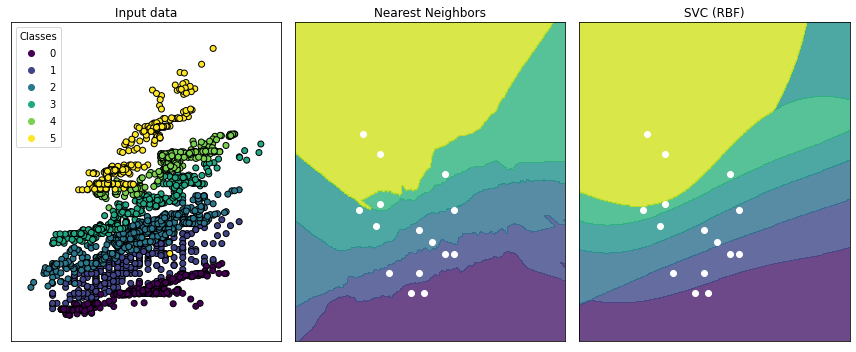
\includegraphics[scale=0.5]{graf.png}
    \caption{Gráfica con las fronteras de decisión y los puntos de prueba correspondientes.}
    \label{fig:graph}
\end{figure}

Observamos que la rotunda mayoría de los puntos de prueba definidos anteriormente en el código, entran cada uno en la zona de la clase que le corresponde. Con lo cual podemos afirmar que los algoritmos implementados aprendieron correctamente la clasificación de la obesidad con las etiquetas de clase y el entrenamiento brindado por nosotros.

\subsection{Conclusión}
Los métodos del machine learning son una herramienta muy útil para el análisis de datos, pues resuelven diversos tipos de problemas, como la clasificación en este caso, sin sujetarse a la subjetividad de los parámetros que recibe, con esto me refiero a que en casos donde utilizar una formula como la del IMC no es la manera mas adecuada para clasificar, sino que hay que considerar otros factores categóricos, el uso de este tipo de métodos permite utilizar estos factores y hacer una clasificación precisa.

\section{Conclusión General}
El análisis de datos puede ser una tarea tediosa y laboriosa, ya que las bases de datos suelen tener miles hasta cientos de miles de instancias, el uso de herramientas para su análisis como lo son \textit{Excel} o \textit{Python} permite utilizar librerías mas especializadas para realizar mas eficientemente los análisis, la necesidad que buscan cubrir estos análisis pueden ser tan especificas como generales y para mi, ahí está la ventaja de utilizar un lenguaje de programación antes que otro tipo de herramienta, como dijo alguna vez una persona muy sabia: "si puedes imaginarlo, puedes programarlo" (Alejandro Taboada "Programacion ATS", 1997-2019).

\begin{thebibliography}{}
\bibitem{Data} G. Rojas Peña, \textit{Estadística de Padrón Electoral y Lista Nominal de Electores}, México: Instituto Nacional Electoral, 2020. Consultado en: 6 de Junio, 2021. [En línea]. Disponible en: https://portal.ine.mx/transparencia/datos-abiertos/\#/archivo/estadistica-padron-electoral-lista-nominal-electores

\bibitem{pag} A. Menon. (2018, Sep 24). Linear Regression in 6 lines of Python [Online]. Available: https://towardsdatascience.com/linear-regression-in-6-lines-of-python-5e1d0cd05b8d

\bibitem{obs} F. Mendoza, & A. de la Hoz, \textit{Dataset for estimation of obesity levels based on eating habits and physical condition in individuals from Colombia, Peru and Mexico}, 2019. Consultado en: 27 de abril, 2021. [En línea]. Disponible en: \url{https://archive.ics.uci.edu/ml/datasets/Estimation+of+obesity+levels+based+on+eating+habits+and+physical+condition+ }

\bibitem{lib} T. M. Mitchell, \textit{Machine learning}. New York, N.Y: MacGraw-Hill, 1997. 

\bibitem{kn} Na8, “Clasificar con K-Nearest-Neighbor ejemplo en Python,” Aprende Machine Learning, 10-Jul-2018. [En línea]. Disponible en: https://www.aprendemachinelearning.com/clasificar-con-k-nearest-neighbor-ejemplo-en-python/. [Consultado en: 16-Jun-2021]. 
\end{thebibliography}

\end{document}
